\section{Ausgangslage}
\label{sec:Ausgangslage}

\begin{wrapfigure}{l}{0.55\textwidth}
  \begin{center}
    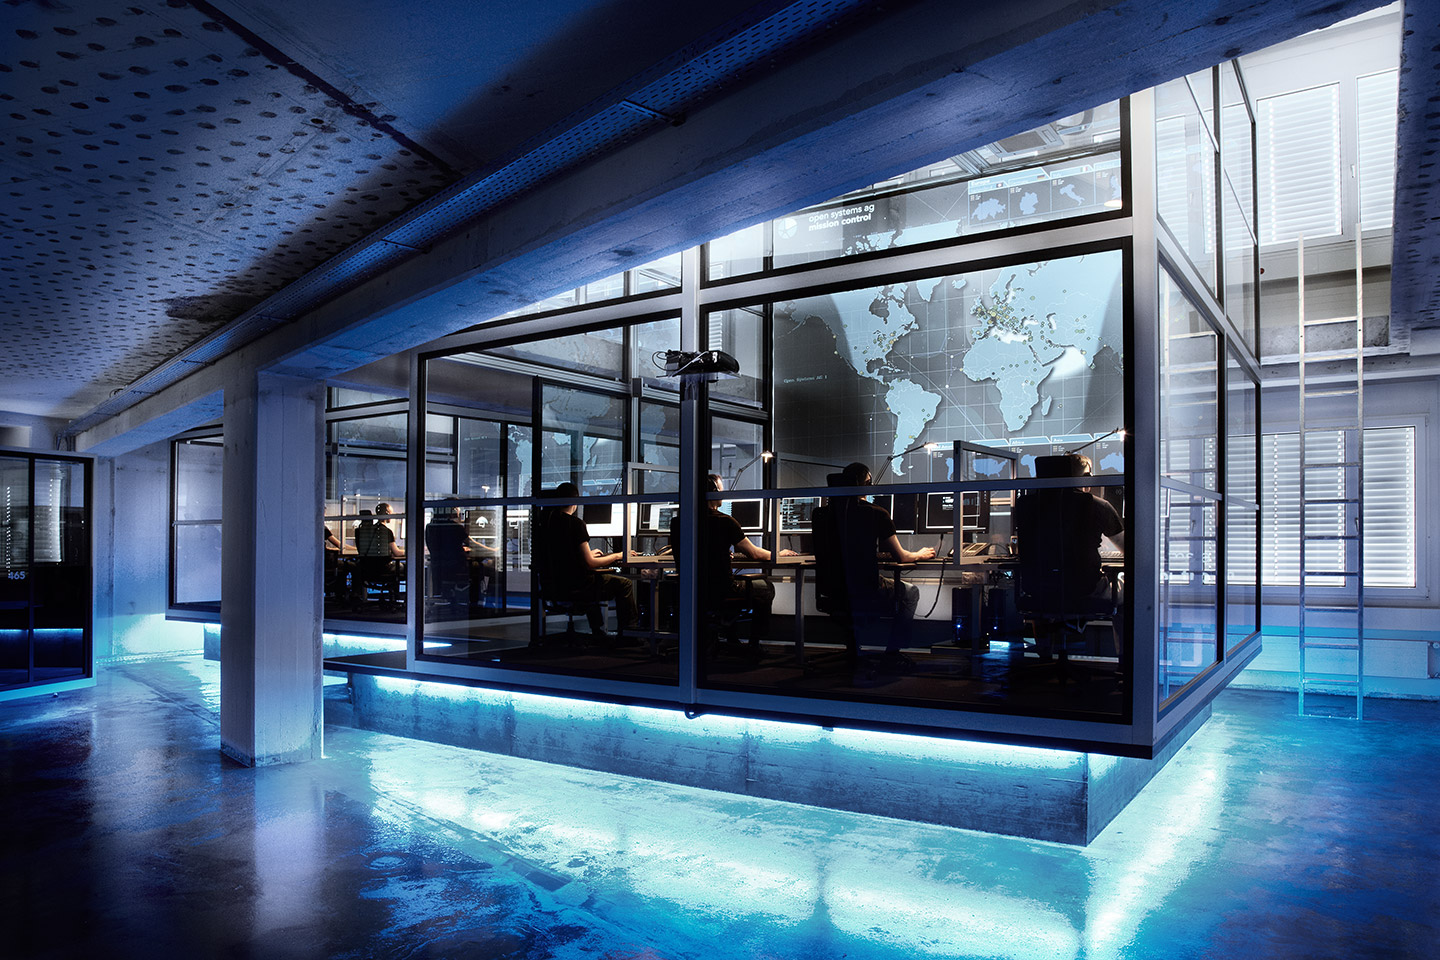
\includegraphics[clip,scale=0.15]{mainpart/anforderungen/img/gallery_mc_01}
    \caption{Mission Control Center}
  \end{center}
\end{wrapfigure}

Die Firma \osag betreibt ein weltweites Netz von \acs{IPsec} \acs{VPN} Verbindungen. Die Kunden der \osag kommen unter anderem aus den Branchen: Finanzen, Versicherungen, Regierung sowie Detail Handel. Daher ist es für \osag sehr wichtig, dass die Verbindungen konstant überwacht werden. Zu diesem Zweck wird auch ein Mission Control Center betrieben dass den Betrieb der \acs{VPN} Tunnels 24/7 überwacht. Dieses Mission Control Center\footnotemark[1] ist zuständig, dass periodische Tests der Verbindungsqualität gemacht werden sowie akute Probleme direkt erkannt und behoben werden. Das manuelle Überprüfen von Paket-Verlusten und bestimmen von Fragmentierungsproblem nimmt viel Zeit in Anspruch. Es soll nun eine Applikation programmiert werden, womit sich diese Arbeit automatisieren lässt, sodass mit weniger Aufwand eine bessere Verbindungsqualität gewährleistet werden kann.

\footnotetext[1]{Bild: \url{http://open.ch}}

\subsection{Produktfunktion}
Mit dem Tool soll das Erkennen und Diagnostizieren von Problemen bei \acs{IPsec} \acs{VPN} Verbindungen vereinfacht werden. Dabei soll das \tool{} die Möglichkeit bieten passiv Paket-Verluste zu erkennen sowie aktiv die \acs{MTU} zu bestimmen. Die Applikation ist als konstant laufender Service konzipiert und bietet daher keine graphische Oberfläche sondern nur ein Commandline-Interface. Für die Kommunikation mit den Benutzern des Tools sollen Log-Einträge verwendet werden.

\subsection{Benutzercharakteristik}
Die Benutzer des \tool{} sind Netzwerkadministratoren und Entwickler die \acs{IPsec} \acs{VPN} Tunnels betreiben. Daher kann ein gutes Mass an technischem Verständnis und Erfahrung bei der Verwendung von Commandline-Applikationen gerechnet werden.

\subsection{Abhängigkeiten}
Das \tool{} ist grundsätzlich eine eigenständige Applikation. Es wurde jedoch bereits in der Ausschreibung dieser Arbeit festgelegt dass libpcap als Library für das Capturen von Paketen verwendet werden soll. Daher ist das \tool{} von libpcap und einem entsprechenden Wrapper abhängig.